\documentclass{standalone}
\usepackage{tikz}
\usepackage{tkz-euclide} % pratique pour marquer les angles
\begin{document}
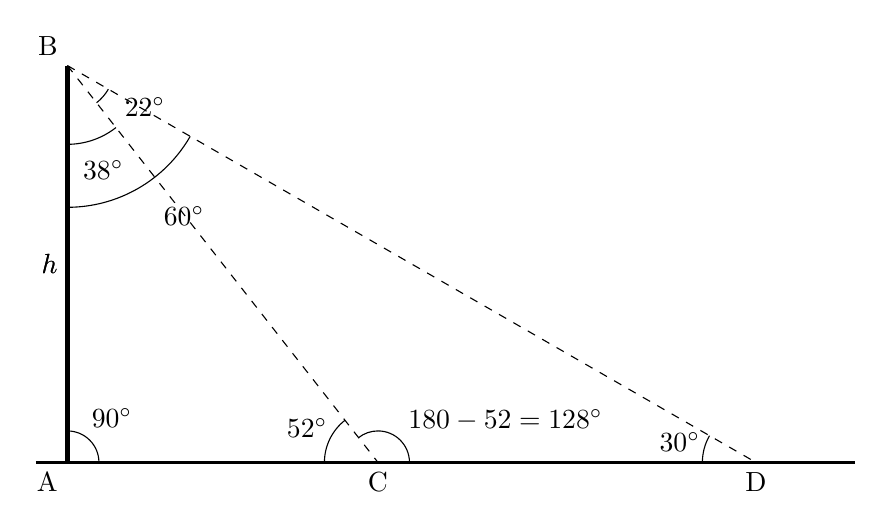
\begin{tikzpicture}[scale=0.4]

  %--- Données (échelle réduite) ---
  \def\h{12.6}       % hauteur arbre (approx)
  \def\sone{9.86}    % ombre pour 52°
  \def\stwo{21.86}   % ombre pour 30°

  %--- Points ---
  \coordinate (A) at (0,0);          % base de l'arbre
  \coordinate (B) at (0,\h);         % sommet de l'arbre
  \coordinate (C) at (\sone,0);      % extrémité de l'ombre à 52°
  \coordinate (D) at (\stwo,0);      % extrémité de l'ombre à 30°

  %--- Sol et arbre ---
  \draw[thick] (-1,0)--(25,0);
  \draw[line width=2pt] (A)--(B);

  %--- Ombres ---
  \draw[dashed] (B)--(C) node[pos=0.5,above,sloped] {};
  \draw[dashed] (B)--(D) node[pos=0.5,above,sloped] {};

  %--- Segments d'ombre ---
  \draw (A)--(C);
  \draw (A)--(D);

  %--- Nom des sommets ---
  \node[below left] at (A) {A};
  \node[above left] at (B) {B};
  \node[below] at (C) {C};
  \node[below] at (D) {D};

  %--- Angles marqués à A ---
  %--- Angles marqués à A ---
  \tkzMarkAngle[size=1cm](C,A,B)  % angle 52
  \tkzLabelAngle[pos=2](C,A,B){$90^\circ$}

  \tkzMarkAngle[size=1.7cm](B,C,A) % angle 30
  \tkzLabelAngle[pos=2.5](B,C,A){$52^\circ$}

  \tkzMarkAngle[size=1.7cm](B,D,A) % angle 30
  \tkzLabelAngle[pos=2.5](B,D,A){$30^\circ$}

  \tkzMarkAngle[size=1.cm](D,C,B) % angle 30
  \tkzLabelAngle[pos=1.5, right](D,C,B){$180-52=128^\circ$}

  \tkzMarkAngle[size=2.5cm](A,B,C) % angle 30
  \tkzLabelAngle[pos=3.5](A,B,C){$38^\circ$}

  \tkzMarkAngle[size=1.5cm](C,B,D) % angle 30
  \tkzLabelAngle[pos=2, right](C,B,D){$22^\circ$}

  \tkzMarkAngle[size=4.5cm](A,B,D) % angle 30
  \tkzLabelAngle[pos=5.5, right](A,B,D){$60^\circ$}

  %--- Annotation de la hauteur ---
  \node[left] at ($(A)!0.5!(B)$) {$h$};

  %--- Annotation différence d'ombre ---
  %\draw[<->] (C,-1.2) -- (D,-1.2) node[midway,below] {$\Delta s=12{,}0$ m};



  %--- Annotation de la hauteur ---
  \node[left] at ($(A)!0.5!(B)$) {$h$};

  %--- Annotation différence d'ombre ---
 % \draw[<->] (C,-1.2) -- (D,-1.2) node[midway,below] {$\Delta s=12{,}0$ m};

\end{tikzpicture}
\end{document}
